\begin{frame}
  \frametitle{Object Interactions \only<4>{ ... via remote method invocations}}
  \begin{figure}
%so far we only spoke abt units of state in the app
%and expressing the app in terms of units natural to the domain
%so we've done that.
	\includegraphics<1>[width=0.9\textwidth]{../figures/progmodel/07-obj-programmer-view.pdf}
%we have this impressive decomposition of data and functionality across collections of objects
%how do you stitch all these objects into a cohesive fabric that makes the app do what its supposed to do
%there's one ingredient that i've avoided mentioning up to this point and those are interactions.
%these obj have to interact with each other
	\includegraphics<2>[width=0.9\textwidth]{../figures/progmodel/05-parallelism-via-obj-collections.pdf}
%in a sequential environment, which all of us are familiar with
%app state is in objects, and app logic / interactions is via method invocations
	\includegraphics<3>[width=0.9\textwidth]{../figures/progmodel/08-seq-obj-methods.pdf}
%charm retains this same modality
%we enable method invocations across process or addr space boundaries
%however with minor modifications from the sequential semantic
	\includegraphics<4>[width=0.9\textwidth]{../figures/progmodel/09-rmi-synchronous.pdf}
  \end{figure}
\end{frame}


\begin{frame}
\frametitle{1. Not every object is remotely invocable}
%we do NOT encourage a notion of a flat global address space, where it magically appears that
%all app entities are in the same address space, and any object can call / interact with anyone else
%instead, we strive to keep the locality information visible to the app
%the first step to that is to permit RMI only on globally visible objects
  \begin{figure}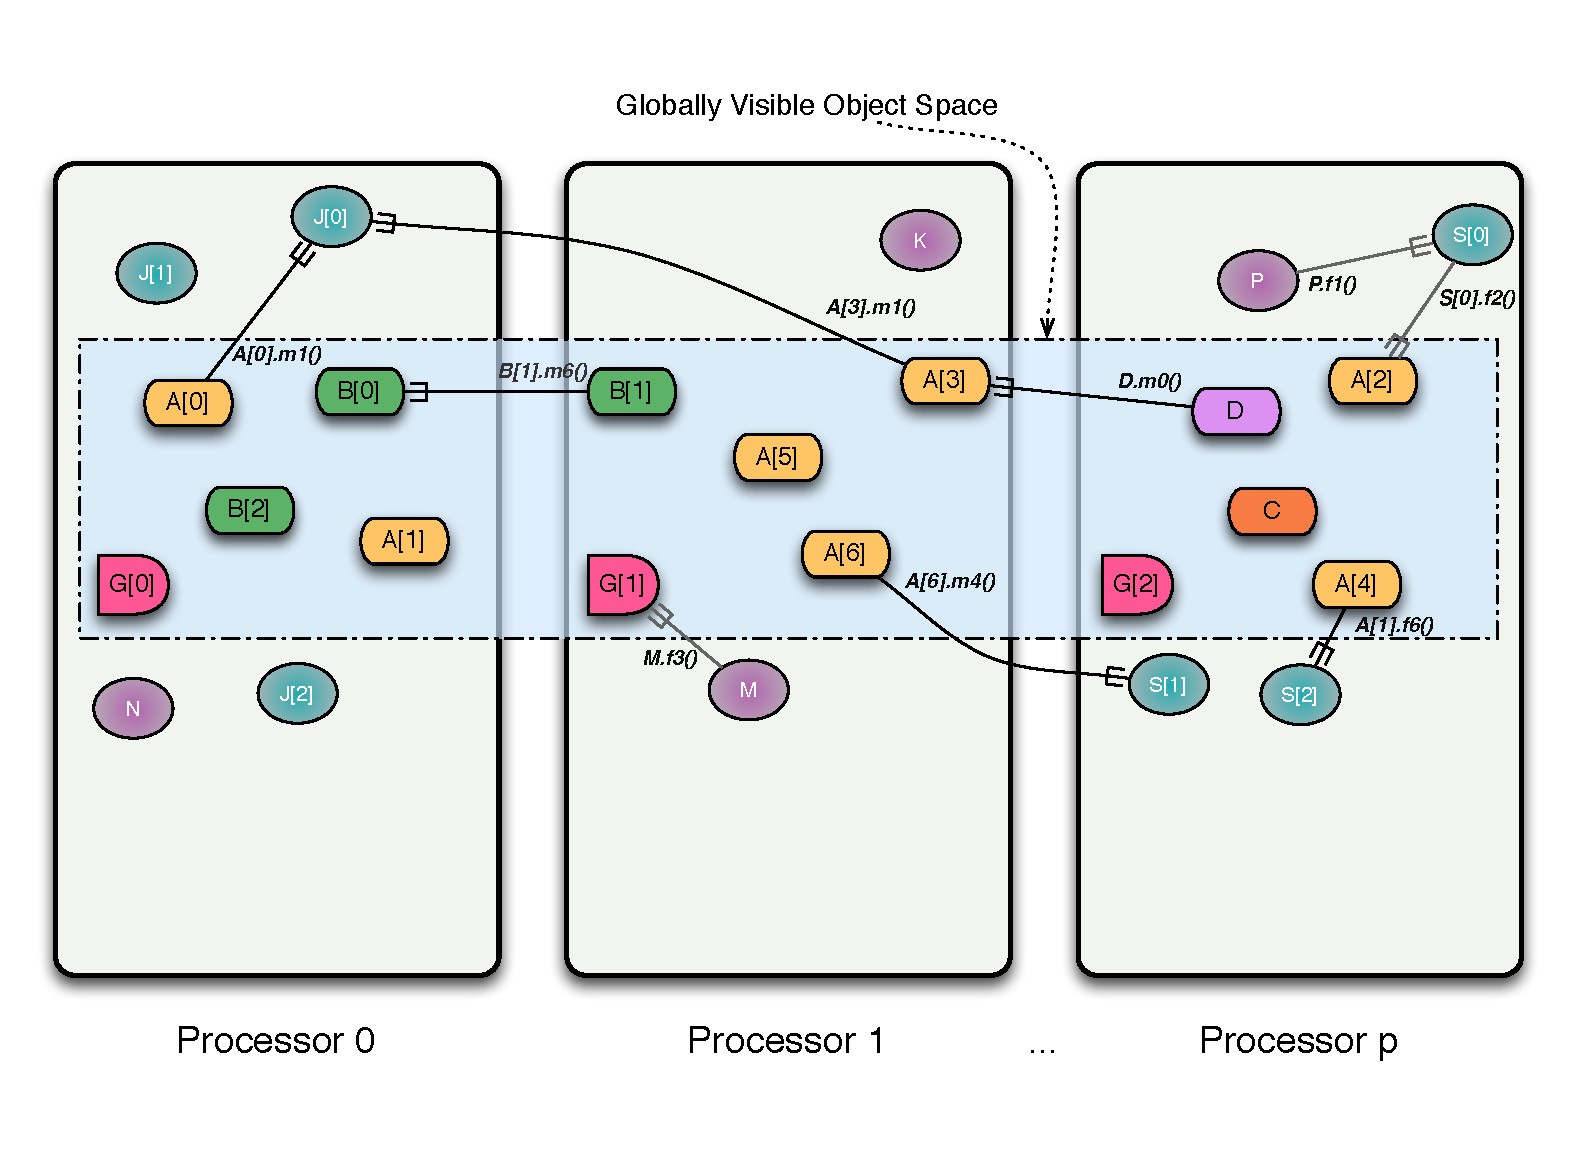
\includegraphics[width=0.9\textwidth]{../figures/progmodel/10-rmi-notgas.pdf}\end{figure}
\end{frame}


\begin{frame}
\frametitle{2. Not every method is remotely invocable}
%only subset of methods elevated into global namespace
%programmer annotates which methods are globally visible
%only globally visible methods can be invoked across proc boundaries
%intro term entry methods. will explain why later.
  \begin{figure}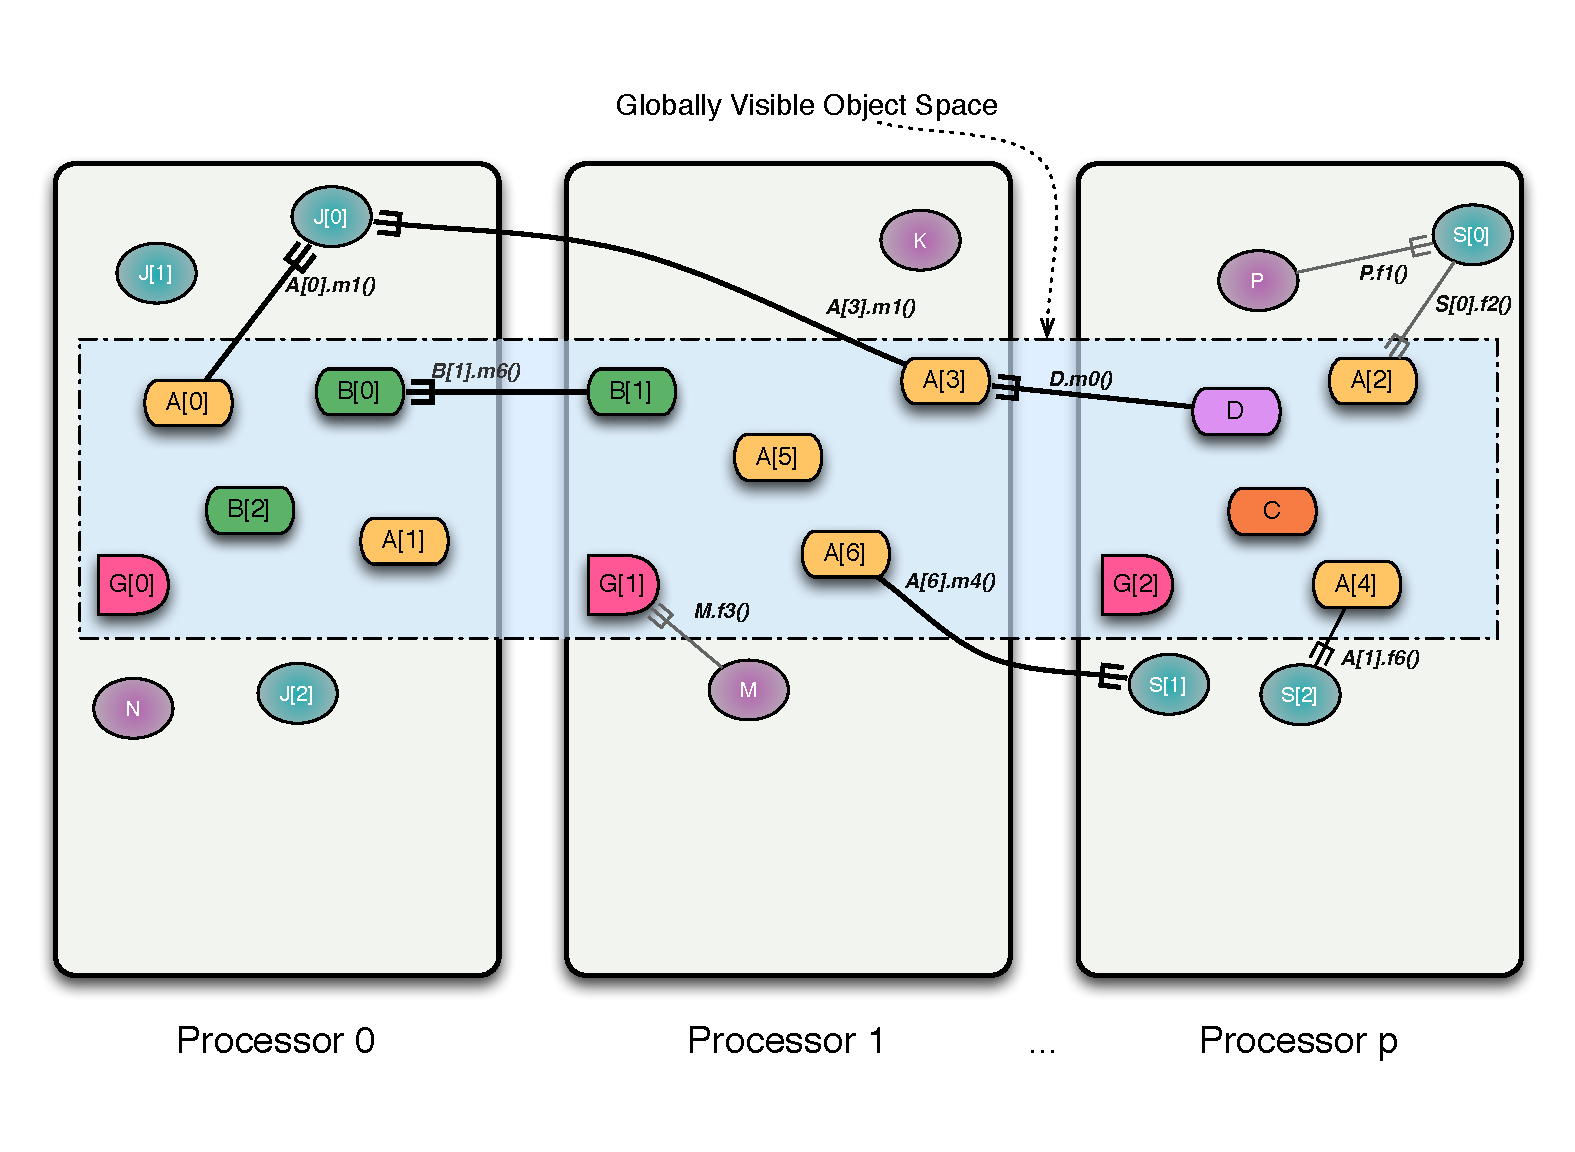
\includegraphics[width=0.9\textwidth]{../figures/progmodel/11-global-methods.pdf}\end{figure}
\end{frame}


\begin{frame}[fragile,t]
\frametitle{Globally Visible \emph{Entry Methods}}
In \texttt{foo.ci}
\begin{lstlisting}
array [2D] Foo {
  entry Foo(int c, double d);
  entry void compute(int count, double[count] data);
};
\end{lstlisting}
In \texttt{foo.h}
\begin{lstlisting}
class Foo : public CBase_Foo {
  int c_; double d_;
public:
  Foo(int c, double d);
  void compute(int count, double * data);
};
\end{lstlisting}
In \texttt{foo.C}
\begin{lstlisting}
Foo::Foo(int c, double d) : c_(c), d_(d) { }
void Foo::compute(int count, double * data)
{ /* . . . */ }
\end{lstlisting}
%
%- ci file entry method syntax
%- proxy call syntax
%
  %\frametitle{Addressing objects is independent of location}
%  proxies. what they are. what they do. generated code.\\
%  typical proxy patterns will hide the very existence of a proxy
%  in that sense, this is not aptly named.
%  here, it is a conscious design decision to make the user code very aware of
%  the existence of the proxy. provides locality info to app programmer.
%  any interaction with a proxy is a possible remote interaction.
%  u can have a local instance of a chare array and access it via pointer. then local object
% but only if local. if its remote, then u have to interact via proxy
\end{frame}

\begin{frame}[fragile]
\frametitle{Calling Entry Methods: Proxy Objects}
\begin{lstlisting}
// Construct a 10*10 array of Foo chares, each initialized with {42, 2.7}
CProxy_Foo f = CProxy_Foo::ckNew(10, 10, 42, 2.7);

double d[7] = {0.0, 1.1, 2.2, 3.3, 4.4, 5.5, 6.6};

// Call Foo::compute(7, d) on the object at (1, 2) in the collection
f(1, 2).compute(7, d);
\end{lstlisting}
Many RMI proxy implementations try to hide remote-ness. Ours draws attention to potential expense of non-local operations.
\end{frame}


\begin{frame}
\frametitle{3. Remote methods are of void return type}
  What happens if an object waits for a return value from a method invocation?
  \pause
  \begin{center}
    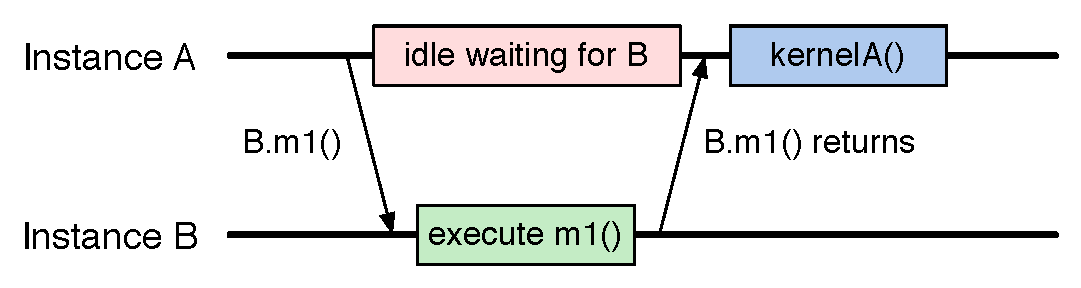
\includegraphics[width=\textwidth]{../figures/objectSequence.pdf}
  \end{center}
  \pause
  \begin{itemize}
    \item Performance
    \item Latency
    \item Reasoning about correctness
  \end{itemize}
\end{frame}


\begin{frame}
\frametitle{3. Remote methods are of void return type}
  \begin{center}
    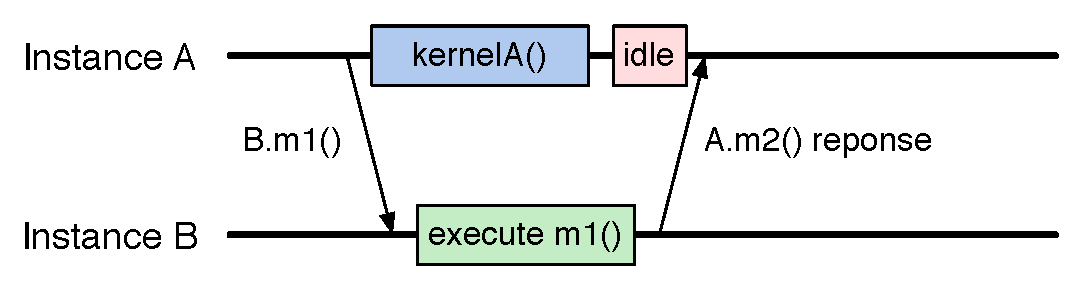
\includegraphics[width=\textwidth]{../figures/objectSequenceAsync.pdf}
  \end{center}
  \begin{itemize}
  \item Hence, method invocations should be asynchronous
    \begin{itemize}
    \item No return values
    \end{itemize}
  \item Computations are driven by the incoming data
    \begin{itemize}
    \item Initiated by the sender or method caller
    \end{itemize}
  \end{itemize}
\end{frame}


\begin{frame}
\frametitle{\only<3-> {Entry Methods}}
	\onslide<2->{ Asynchronous, non-blocking remote method invocations on chares}
	\begin{center}
        \includegraphics<1>[width=0.9\textwidth]{../figures/progmodel/11-global-methods.pdf}
        \includegraphics<2->[width=0.9\textwidth]{../figures/progmodel/12-async-nonblock-rmi.pdf}
	\end{center}
\end{frame}



\begin{frame}
\frametitle{How do you get return values}
	\begin{center}
        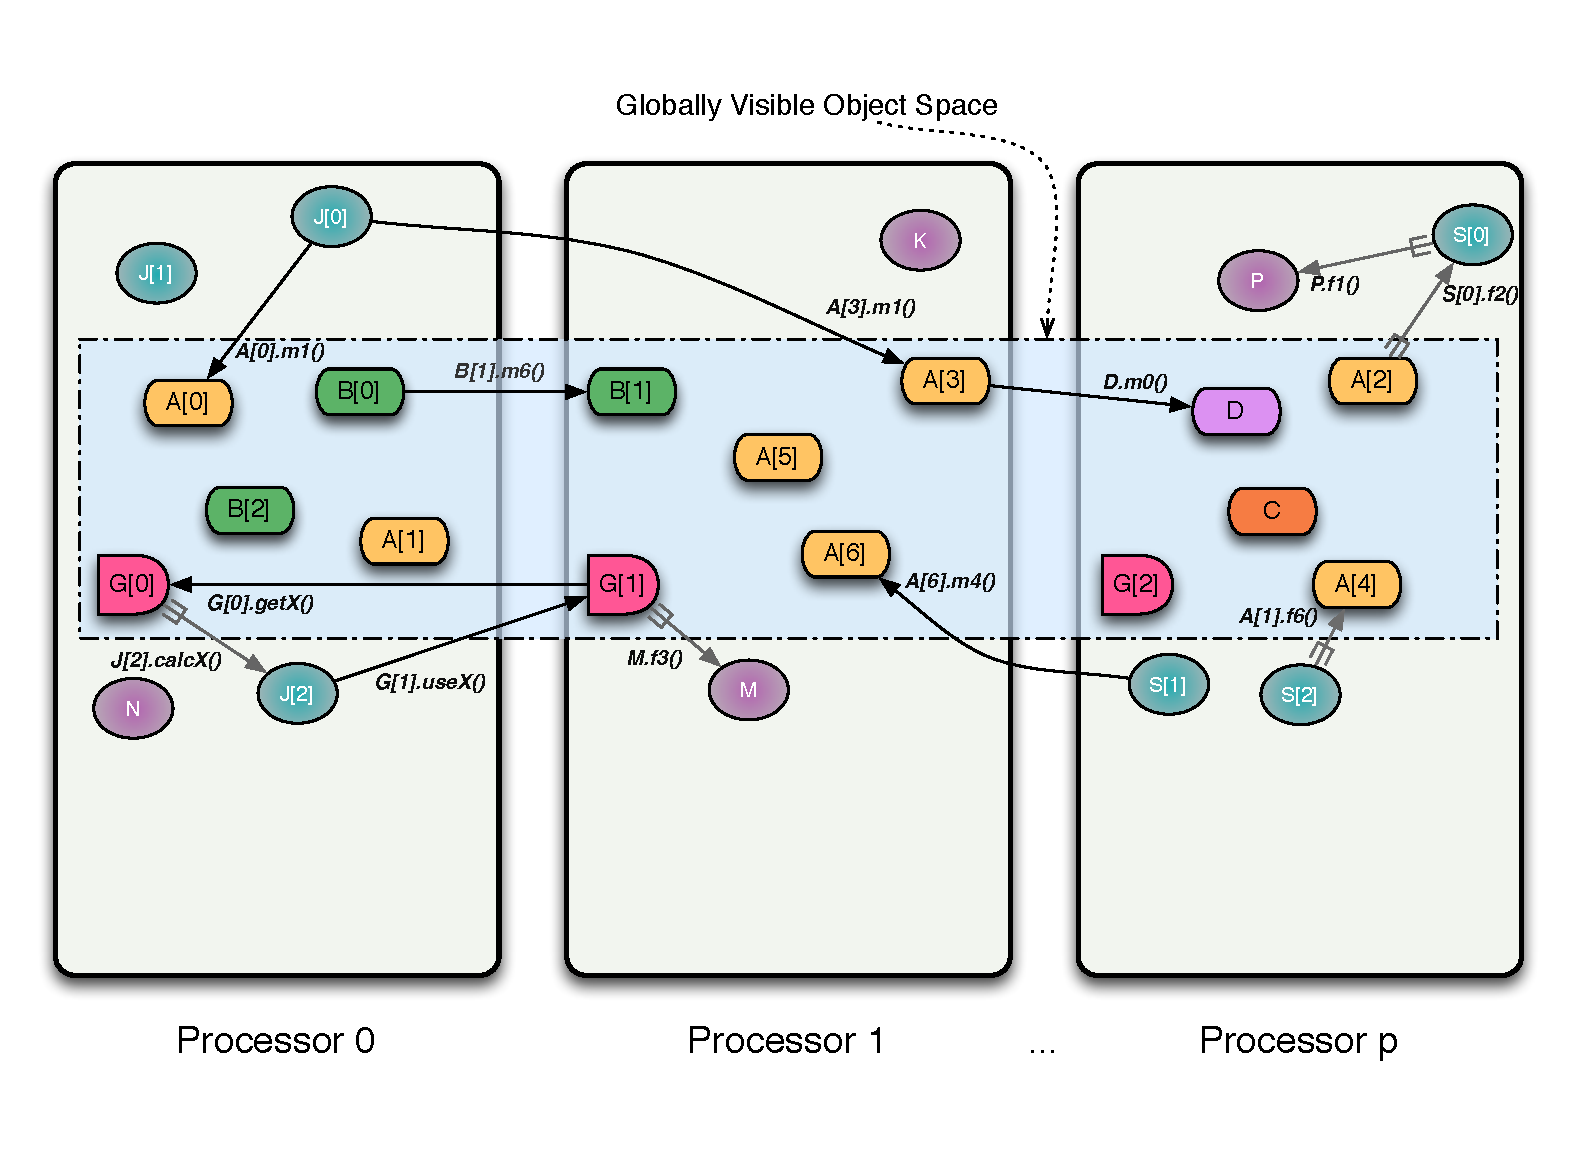
\includegraphics[width=0.9\textwidth]{../figures/progmodel/13-rmi-return-values.pdf}
	\end{center}
\end{frame}


\begin{frame}
\frametitle{Method invocation on object collections}
	\begin{center}
        \includegraphics<1>[width=0.9\textwidth]{../figures/progmodel/13-rmi-return-values.pdf}
        \includegraphics<2>[width=0.9\textwidth]{../figures/progmodel/14-rmi-collective.pdf}
	\end{center}
\end{frame}


\begin{frame}
\frametitle{Entry methods and Dataflow}
    \begin{itemize}[<+->]
        \item void return types imply one-way information transfer
        \item signal application's intent to perform (possibly) remote task
        \item carry required input data for remote task
        \item express parallel dependencies
    \end{itemize}
\end{frame}


\begin{frame}
\frametitle{Biomolecular Physics: NAMD}
\framesubtitle{Parallel decomposition and dependencies}
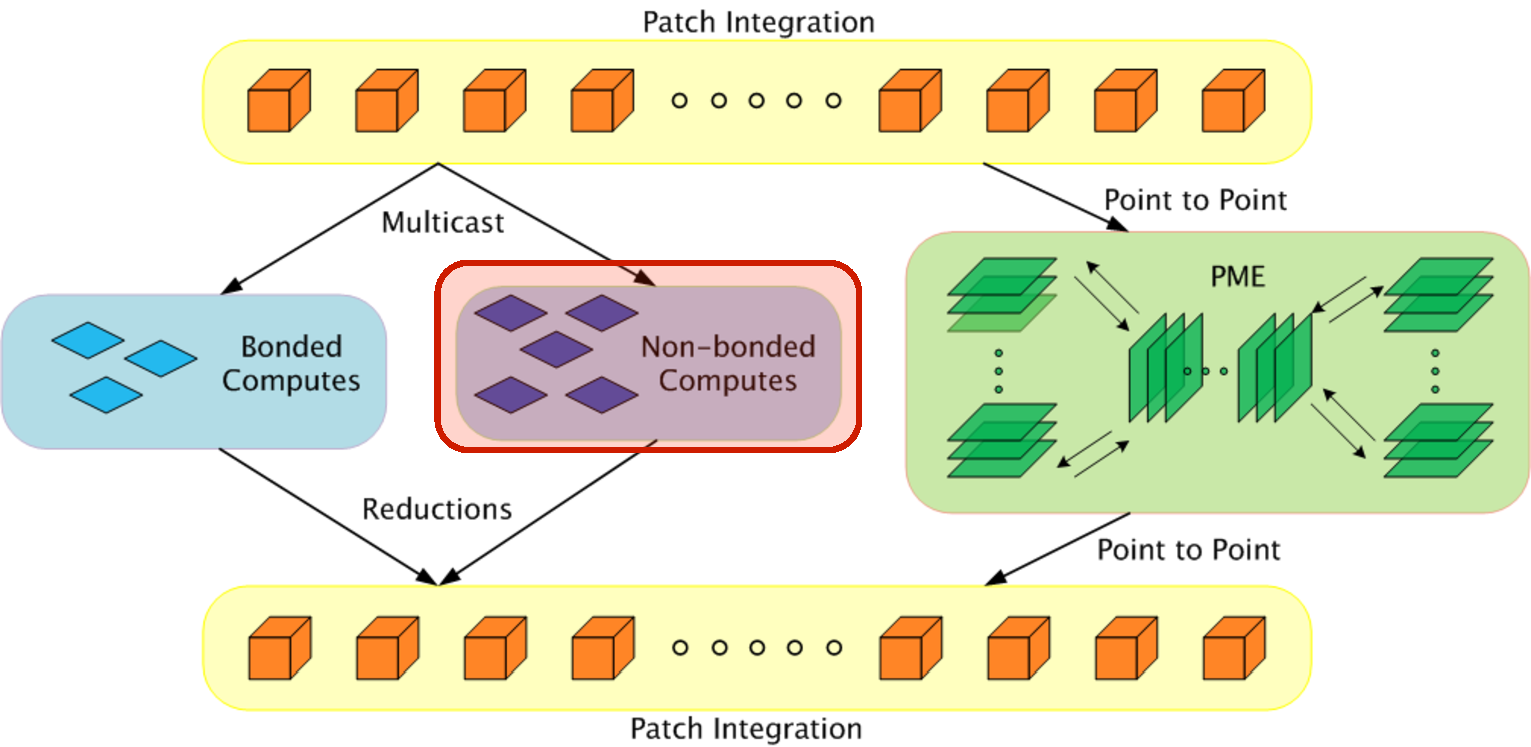
\includegraphics[width=\textwidth]{../figures/md_parallelize.pdf}
\end{frame}


{
\usebackgroundtemplate{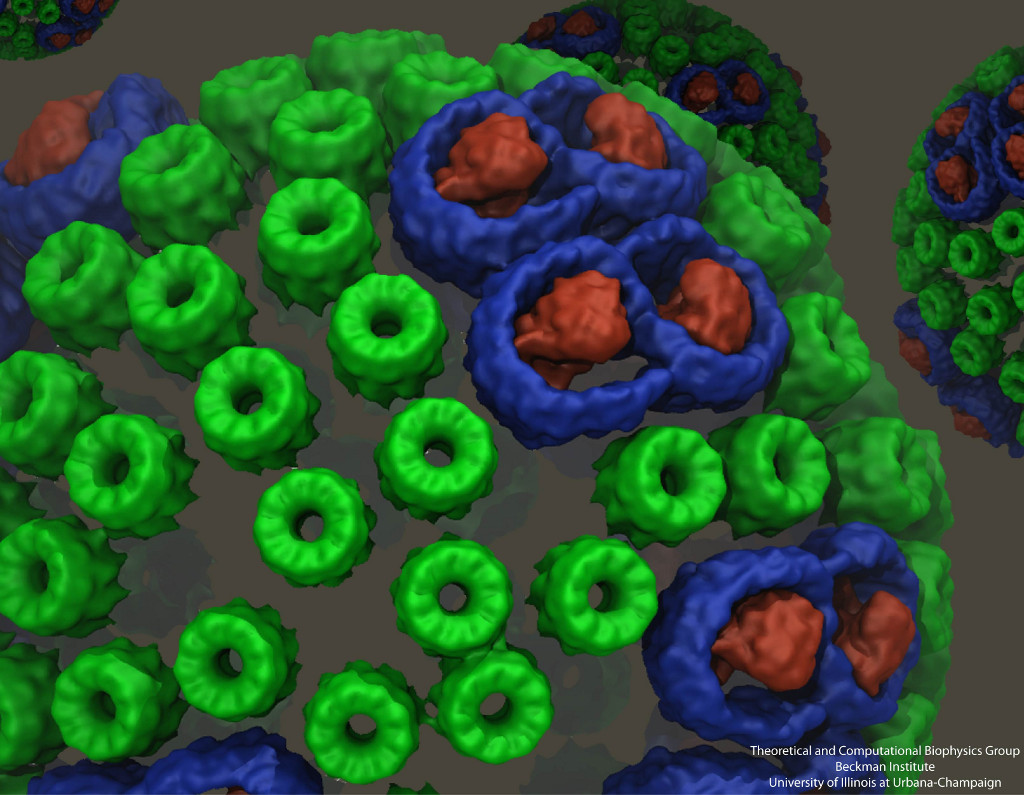
\includegraphics[width=\paperwidth]{../figures/namd/chromatophore-vesicle-2012-01.jpg}}
\begin{frame}
\frametitle{Biomolecular Physics: NAMD}
\framesubtitle{Chromatophore vesicle in purple bacteria}
\end{frame}
}


\begin{frame}
\frametitle{Biomolecular Physics: NAMD}
\framesubtitle{ApoA1 on IBM BlueGene P/Q (Intrepid/Mira)}
\onslide<2>{794 us / step}
\begin{center}
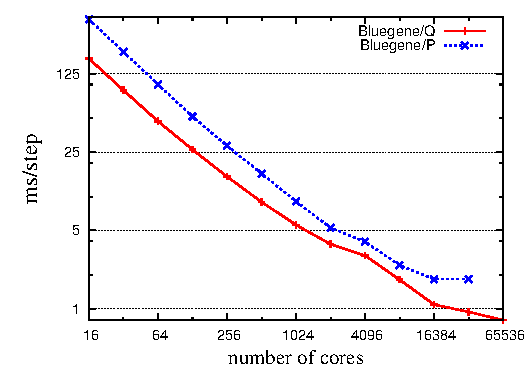
\includegraphics[width=0.9\textwidth]{../figures/apoa1-pme4-PQ.pdf}
\end{center}
\end{frame}


\begin{frame}
\frametitle{Biomolecular Physics: NAMD}
\framesubtitle{100M atom STMV on Cray XK6 (Titan)}
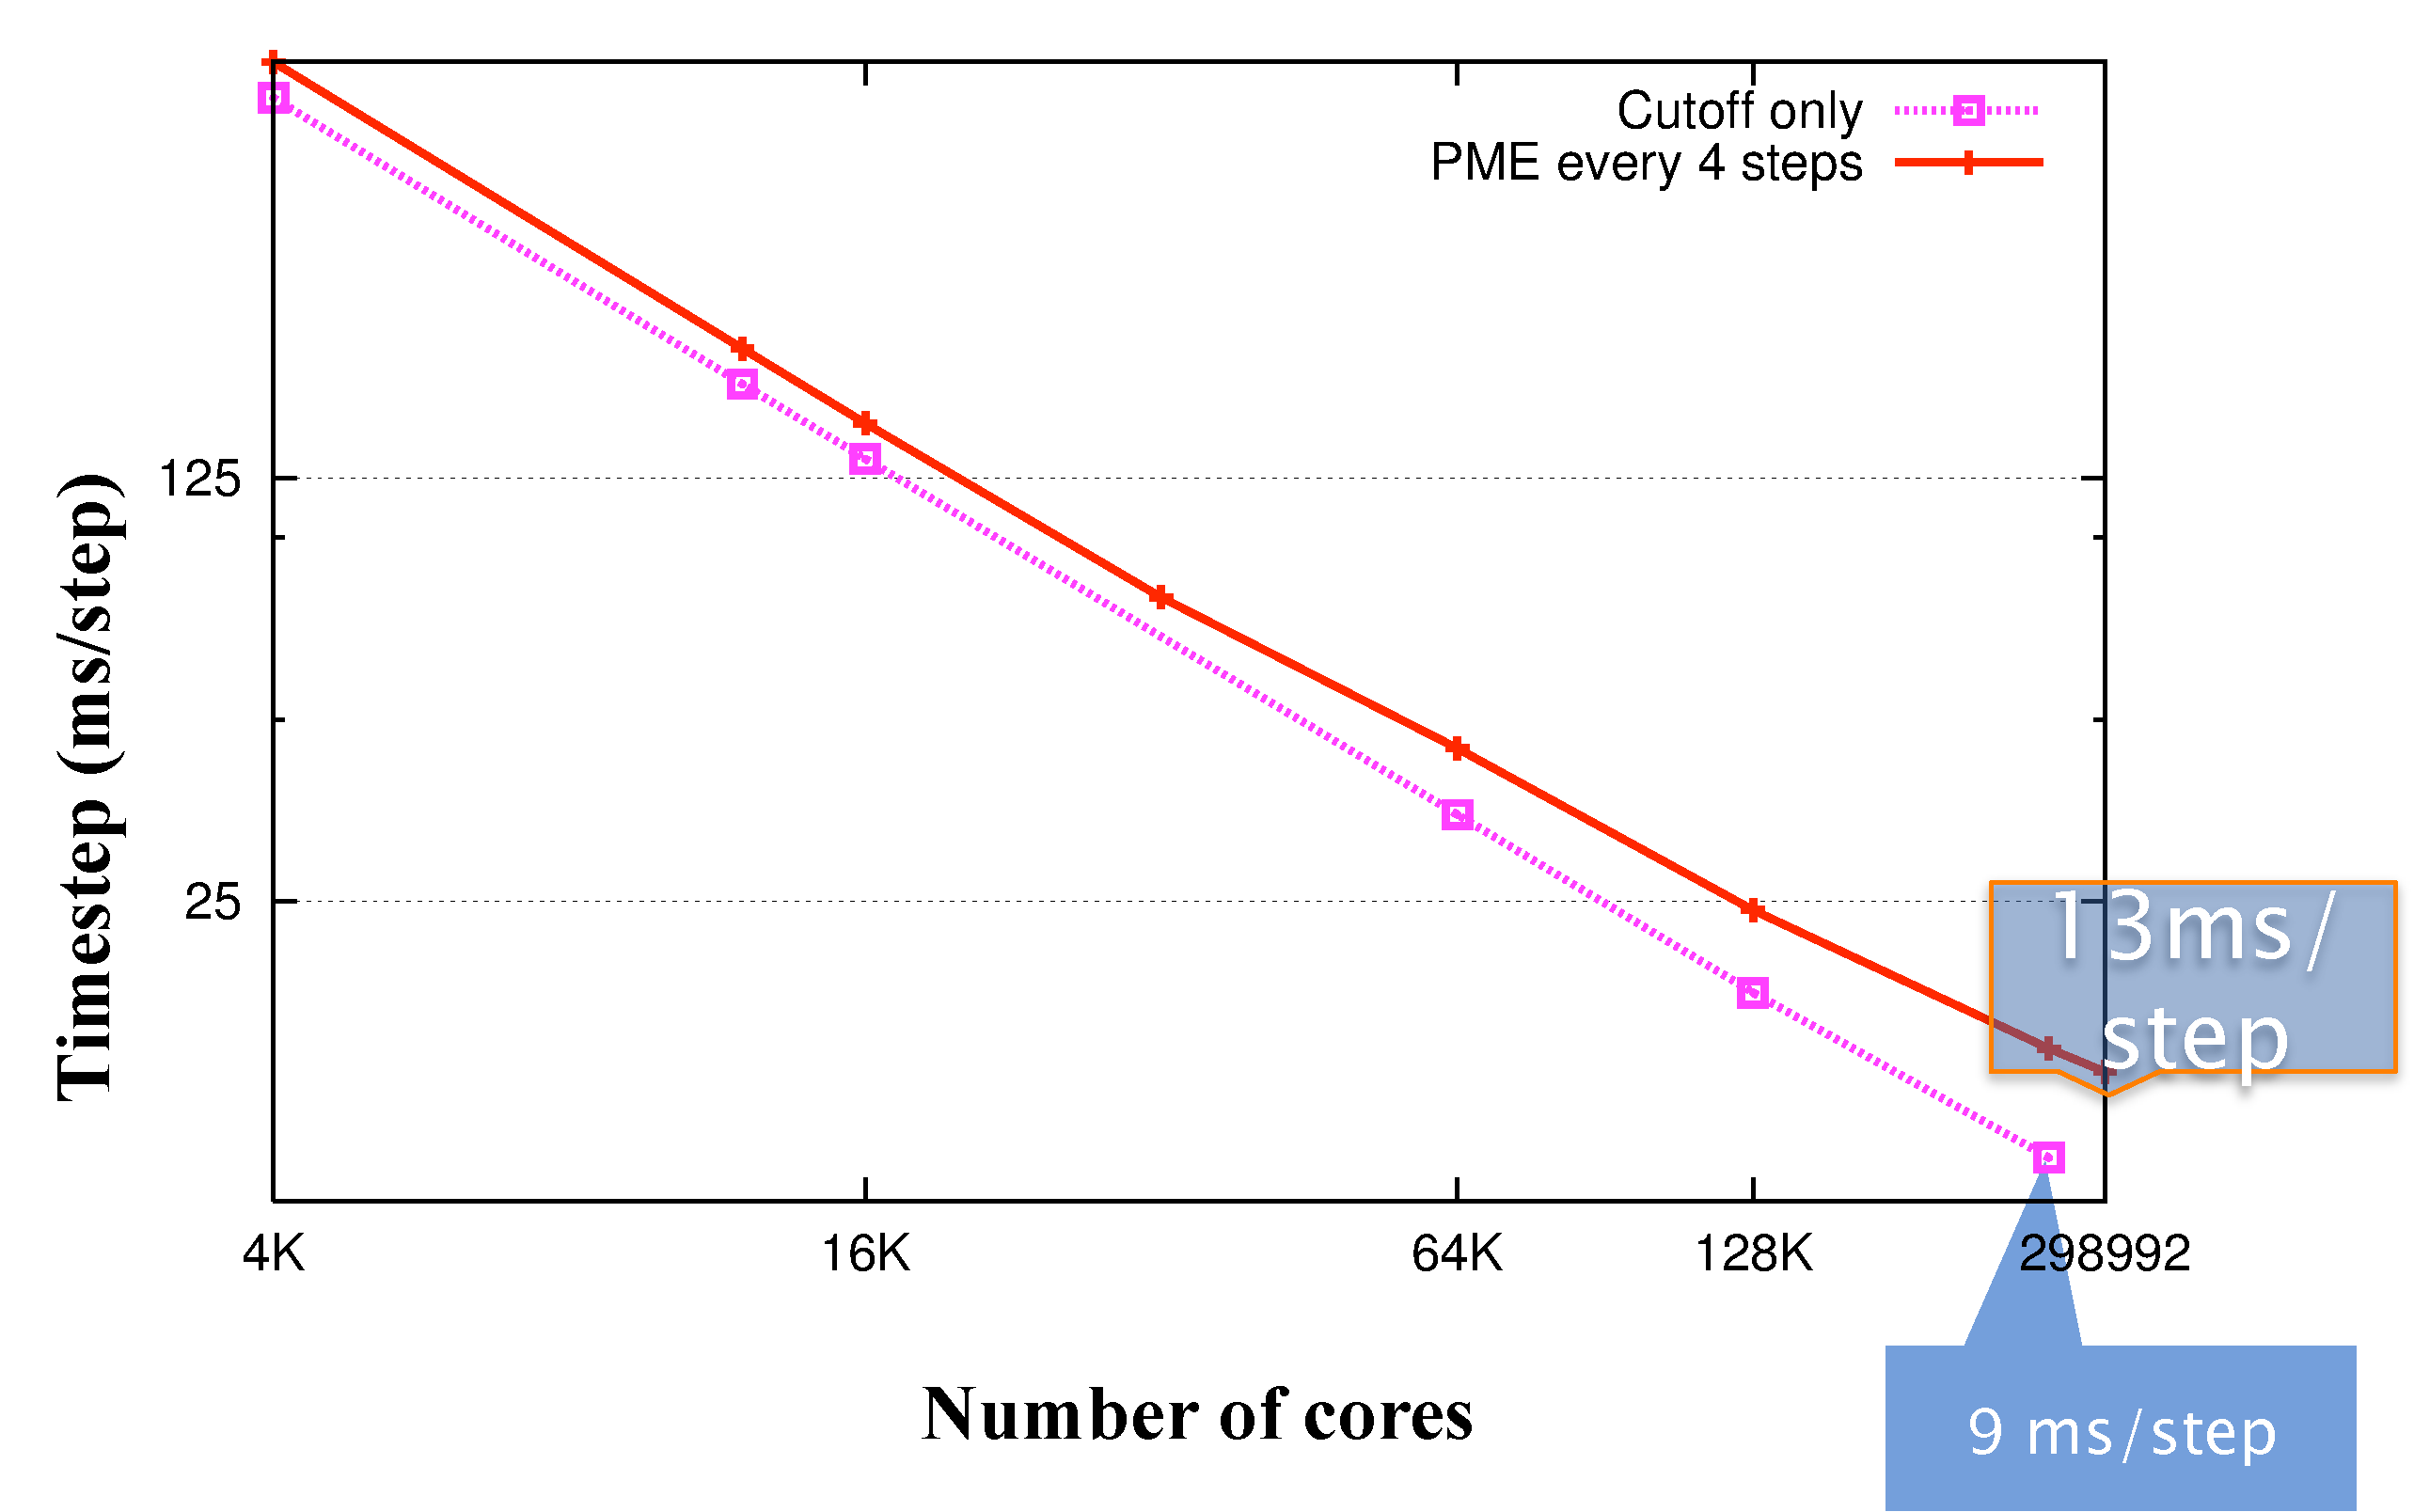
\includegraphics[width=0.9\textwidth]{../figures/namd_titan.pdf}
\end{frame}


